%%%%%%%%%%%%%%%%%%%%%%%%%%%%%%%%%%%%%%%%%%%%%%%%%%%%%%%%%%%%%%%%%%%%%%%%%%%%%%%
%%%%%%%%%%%%%%%%%%%%%%%%%%%%%%%%%%%%%%%%%%%%%%%%%%%%%%%%%%%%%%%%%%%%%%%%%%%%%%%
%%%%%%%%%%%%%%%%%%%%%%%%%%%%%%%%%%%%%%%%%%%%%%%%%%%%%%%%%%%%%%%%%%%%%%%%%%%%%%%
%
%\begin{figure}[h]
%\centering
%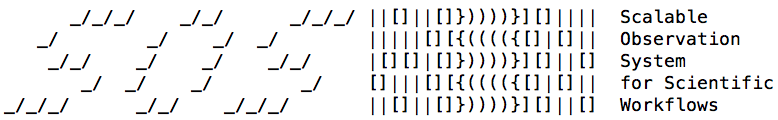
\includegraphics[width=\columnwidth]{images/sosflow_masthead.png}
%\label{fig_masthead}
%\end{figure}
%
%%%%%%%%%%%%%%%%%%%%%%%%%%%%%%%%%%%%%%%%%%%%%%%%%%%%%%%%%%%%%%%%%%%%%%%%%%%%%%%
%%%%%%%%%%%%%%%%%%%%%%%%%%%%%%%%%%%%%%%%%%%%%%%%%%%%%%%%%%%%%%%%%%%%%%%%%%%%%%%
%%%%%%%%%%%%%%%%%%%%%%%%%%%%%%%%%%%%%%%%%%%%%%%%%%%%%%%%%%%%%%%%%%%%%%%%%%%%%%%
\section{Introduction}
%
Modern clusters for parallel computing are complex environments.
%
High-performance applications that run on modern clusters do so often with
little insight about their or the system's behavior.
%
This is not to say that information is unavailable. 
%
After all, sophisticated parallel measurement systems can capture performance and
power data for characterization, analysis, and tuning purposes, but
the infrastructure for observation of these systems is not intended
for general use.
%
Rather, it is specialized for certain types of performance information
and typically does not allow online processing.
%
Other information sources of interest might include the
operating system (OS), network hardware, runtime services, or the
parallel application itself.
%
Our general interest is in parallel application monitoring: the
observation, introspection, and possible adaptation of an application
during its execution.
%
\par
%
Application monitoring has several requirements.
%
%Because information could come from different sources and be used for
%different purposes, it is important to have a flexible means for
%information to be provided from both the application and the system
%environment.
%
It is important to have a flexible means to gather information from
different sources on each node --- primarily the application and
system environment.
%
%Because information will need to be processed online, it is important
%to enable analysis in situ with the application.
%
Additionally, for the gathered information to be processed online,
analysis will need to be enabled in situ with the application
\cite{da2014architecture}.
%
%Because analysis can result in application feedback, query and control
%interfaces are required, again to both the application and the system.
%
Query and control interfaces are required to facilitate
an active application feedback process.
%
The analysis performed can be used to give feedback to both the
application, the operating environment, and performance tools.
%
There exists no general purpose infrastructure that can be programmed,
configured, and launched with the application to provide the
integrated observation, introspection, and adaptation support
required.
%
\par
%
This paper presents the \textit{Scalable Observation System (SOS)} for
integrated application monitoring.
%
A working implementation of SOS is contributed as a part of this
research effort, \textit{SOSflow}.
%
The SOSflow platform demonstrates all of the essential characteristics
of the SOS model, showing the scalability and flexibility inherent to
SOS with its support for observation, introspection, feedback, and
control of scientific workflows.
%
The SOS design employs a data model with distributed
information management and structured query and access.
%
A dynamic database architecture is used in SOS to support aggregation
of streaming observations from multiple sources.
%
%SOS provides interfaces for sources of information to encode data along
%with its context and meaning.
%
Interfaces are provided for in situ analytics to acquire
information and then send back results to application actuators
and performance tools.
%
SOS launches with the application, runs along side it, and can acquire
its own resources for scalable data collection and processing.
%
%

\subsection{Scientific Workflows} %-------------------------------------------%
%
Scientific workflows feature two or more components that are coupled
together, operating over shared information to produce a cumulative
result.
%
These components can be instantiated as lightweight threads belonging
to a single process, or they may execute concurrently as independent
processes.
%
Components of workflows can be functionally isolated from each
other or synchronously coupled and co-dependent.
%
\begin{figure}[h]
\centering
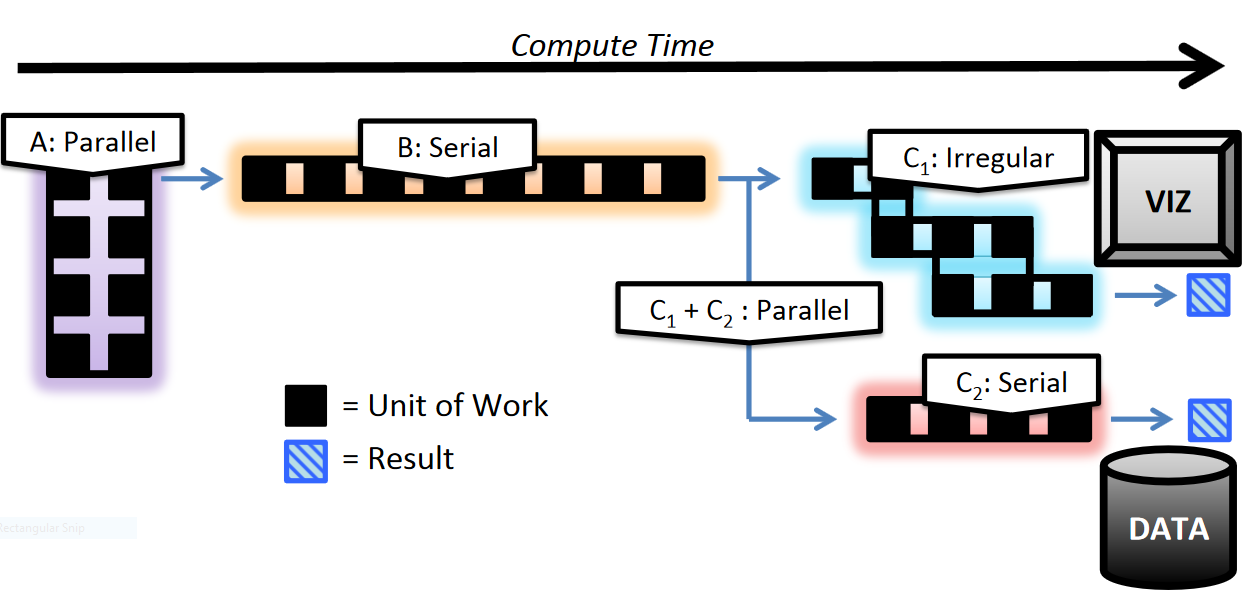
\includegraphics[width=\columnwidth]{images/workflow_example.png}
\caption{Applications Coupled Together Into a Workflow}
\label{fig_workflow_example}
\end{figure}
%
Some workflows can be run on a single node, while others are typically
distributed across thousands of nodes.
%
Additionally, parts of workflows may even be dynamically instantiated and
terminated.
%
The computational profile of a workflow can change between invocations
or even during the course of one execution.
%
%Any general solution for monitoring workflows will need to be capable
%of contextualizing the information processesed by any single
%component, in a scope that can contain and adequatelty contexualize
%the union of all other component scopes.
%
%\par
%
%This research contributes a general solution to the monitoring
%challenges posed by scientific workflows.
%
%To address the general case, SOSflow operates independently of any
%given component and the technology employed to couple components into
%a workflow.
%
%SOSflow's behavior is not bound by the nature of the workflows it
%operates alongside, and by design SOSflow is not limited to a specific
%scale or execution environment.
%
%This particular research effort focuses on three aspects of SOSflow:
%
%\begin{itemize}
%\item \textbf{On-line Ca}
%\item \textbf{Scalable Architecture}
%\item \textbf{Global Information Space}
%\end{itemize}
%
%
%No extant software system adequately expressed all of the properties
%required for the SOSflow model, motivating its development and
%contribution as a novel software artifact.
%
%
%A key feature of SOSflow is its ability to capture and integrate information
%from multiple perspectives simultaneously.
%
\subsection{Multiple Perspectives} %------------------------------------------%
%
\textit{Application state and events} can be sent to SOS from
within the application at any point during its execution.
%
Developers can instrument their programs to be efficiently self-reporting
the data that is relevant to their overall performance, such as progress
through specific phases of a simulation.
%
\par
%

Application performance can be dramatically impacted by changes in
\textit{the state of the operating environment} that is hosting it.
%
The effects of contention for shared resources by multiple concurrent
tasks can be discovered when the events of concurrent tasks are fixed
into a common context for reasoning about their individual and
combined performance.
%
SOS's distributed in situ design is well-suited for capturing
perspective of the global state of a machine.
%
By co-locating the observation system with the workflow components
that are observed, SOS improves the fidelity of system performance
data without requiring the costly delays of synchronization or
congesting the shared network and filesystem resources in use by
applications.
%
\par
%
Many existing \textit{performance tools can provide useful
  observations} at runtime of applications, libraries, and the system
context.
%
The low-level timers, counters, and machine-level data points provided
by specialized performance tools can be a valuable addition to the
higher-level application and system data.
%
\subsection{Motivation}
%
Observing and reasoning about the performance of workflows on
\textit{exascale computational platforms} presents new challenges.
%
Exascale systems will be capable of more than a billion billion
calculations per second, a factor of between 50 to 100 times
faster than present day machines.
%
The physical scale and complexity of exascale machines is expected to
grow by similar factors as its computational speed, motivating a model
that can scale to the same extent.
%
%




%%%
%%%  EOF
%%%

